\PassOptionsToPackage{unicode=true}{hyperref} % options for packages loaded elsewhere
\PassOptionsToPackage{hyphens}{url}
%
\documentclass[12pt,a5paper,]{article}
\usepackage{lmodern}
\usepackage{amssymb,amsmath}
\usepackage{ifxetex,ifluatex}
\usepackage{fixltx2e} % provides \textsubscript
\ifnum 0\ifxetex 1\fi\ifluatex 1\fi=0 % if pdftex
  \usepackage[T1]{fontenc}
  \usepackage[utf8]{inputenc}
  \usepackage{textcomp} % provides euro and other symbols
\else % if luatex or xelatex
  \usepackage{unicode-math}
  \defaultfontfeatures{Ligatures=TeX,Scale=MatchLowercase}
\fi
% use upquote if available, for straight quotes in verbatim environments
\IfFileExists{upquote.sty}{\usepackage{upquote}}{}
% use microtype if available
\IfFileExists{microtype.sty}{%
\usepackage[]{microtype}
\UseMicrotypeSet[protrusion]{basicmath} % disable protrusion for tt fonts
}{}
\IfFileExists{parskip.sty}{%
\usepackage{parskip}
}{% else
\setlength{\parindent}{0pt}
\setlength{\parskip}{6pt plus 2pt minus 1pt}
}
\usepackage{hyperref}
\hypersetup{
            pdftitle={细化政府干预的北京疫情预测},
            pdfauthor={武碧璇 张妍 祁凡 屈亚然 丁晨东},
            pdfborder={0 0 0},
            breaklinks=true}
\urlstyle{same}  % don't use monospace font for urls
\usepackage{graphicx,grffile}
\makeatletter
\def\maxwidth{\ifdim\Gin@nat@width>\linewidth\linewidth\else\Gin@nat@width\fi}
\def\maxheight{\ifdim\Gin@nat@height>\textheight\textheight\else\Gin@nat@height\fi}
\makeatother
% Scale images if necessary, so that they will not overflow the page
% margins by default, and it is still possible to overwrite the defaults
% using explicit options in \includegraphics[width, height, ...]{}
\setkeys{Gin}{width=\maxwidth,height=\maxheight,keepaspectratio}
\setlength{\emergencystretch}{3em}  % prevent overfull lines
\providecommand{\tightlist}{%
  \setlength{\itemsep}{0pt}\setlength{\parskip}{0pt}}
\setcounter{secnumdepth}{5}
% Redefines (sub)paragraphs to behave more like sections
\ifx\paragraph\undefined\else
\let\oldparagraph\paragraph
\renewcommand{\paragraph}[1]{\oldparagraph{#1}\mbox{}}
\fi
\ifx\subparagraph\undefined\else
\let\oldsubparagraph\subparagraph
\renewcommand{\subparagraph}[1]{\oldsubparagraph{#1}\mbox{}}
\fi

% set default figure placement to htbp
\makeatletter
\def\fps@figure{htbp}
\makeatother

\usepackage{ctex}     % 支持中文的标点和章节模式

%\usepackage{xltxtra} % XeLaTeX的一些额外符号
% 设置中文字体
%\setCJKmainfont[BoldFont={黑体},ItalicFont={楷体}]{新宋体}

% 设置边距
\usepackage{geometry}
\geometry{%
  left=2.5cm, right=2.5cm, top=2.5cm, bottom=2.5cm} 

\usepackage{amsthm,mathrsfs} % 基本的ams数学公式
\usepackage{booktabs}        % 增强的表格功能
\usepackage{longtable}       % 支持超过一页的表格

% 下面是自定义的定理环境排版方法
\makeatletter
\def\thm@space@setup{%
  \thm@preskip=8pt plus 2pt minus 4pt
  \thm@postskip=\thm@preskip
}
\makeatother

\title{细化政府干预的北京疫情预测}
\author{武碧璇 张妍 祁凡 屈亚然 丁晨东}
\date{2020-05-28}

\begin{document}
\maketitle

\hypertarget{ux4e00ux6458ux8981}{%
\subsubsection{一、摘要}\label{ux4e00ux6458ux8981}}

  迅速爆发的新型冠状病毒很快蔓延全国,对全国人民带来很大影响。研究预测作为首都的北京市的疫情情况,分析政府干预政策对疫情防控有重大意义。本文利用北京市1月20日-3月26日的疫情数据,选用修正疾病传播率的SIR模型和划分隔离区的SIR模型,对北京市疫情进行预测并与实际对比。结果表明,存在一定程度政府干预的赋权能够有效预测疫情走向,说明政府采取干预政策对疫情防控很有必要。

\textbf{关键词}:北京疫情;SIR模型;预测

\hypertarget{ux4e8cux5f15ux8a00}{%
\subsubsection{二、引言}\label{ux4e8cux5f15ux8a00}}

  本次的新型冠状肺炎是是新中国成立以来在我国发生的传播速度最快、感染范围最广、防控难度最大的一次重大突发公共卫生事件,疫情波及几百个个国家和地区\ldots{}\ldots{}新冠肺炎疫情让世界几乎每个角落都感受到了它的影响。北京作为我们国家的首都和中心城市,是中国的政治、文化、科教和国际交往中心,由于国际疫情形势日益严峻,北京外来人员流动频繁,因此政府对于易感者、感染者以及康复者的这三个人群的防控显得尤为重要,所以研究北京政府干预对于疫情的影响有重大意义。

  接下来,本文将利用北京市1月20-3月26的数据,包括累计确诊人数,累计治愈和累计死亡人数,以及移除人数(累计治愈人数+累计死亡人数),用宋学坤教授团队开发的eSIR包对北京市疫情的转折点做出预测,并将预测结果与实际情况进行对比,寻找政策干预较好的赋权方法,为以后的预测提供一个参照。

\hypertarget{ux4e09ux6d41ux884cux75c5ux6a21ux578bux4ecbux7ecd}{%
\subsubsection{三、流行病模型介绍}\label{ux4e09ux6d41ux884cux75c5ux6a21ux578bux4ecbux7ecd}}

  传染病的基本数学模型,研究传染病的传播速度、空间范围、传播途径、动力学机理等问题,用来指导对传染病的有效地预防和控制。常见的传染病模型按照传染病类型分为
SI、SIR、SIRS、SEIR模型等。

  SI模型适用于疾病不会反复发作的情形,只考虑了传染病爆发和传播的过程。将人群分为
S 类和 I 类,建立如下微分方程:

\(\frac{d S}{d t}=-\beta S I, \quad \frac{d I}{d t}=\beta S I\)

这里β为传染率.在疾病传播期内,所考察地区的总人数 S(t)+I(t) = K 保持不变.

  SIR模型是最著名的流行病模型之一,它具有以下优点:(1)模型简单;
(2)稳定;(3)假设条件相比于其他模型而言偏少;(4)由流量推存量。

  SIRS模型用来刻画治愈后带暂时免疫力的情形。如果所研究的传染病为非致死性的,但康复后获得的免疫不能终身保持,则康复者R可能再次变为易感者S.此时有

\(\frac{d S}{d t}=-\beta S I+\alpha R, \quad \frac{d I}{d t}=\beta S I-\gamma I, \quad \frac{d R}{d t}=\gamma I-\alpha R\)

总人数S(t) + I(t) + R(t) =
N为常数.参数α决定康复者获得免疫的平均保持时间.

  SEIR模型如果所研究的传染病有一定的潜伏期,与病人接触过的健康人并不马上患病,而是成为病原体的携带者,归入E类.此时有:

\(\left\{\begin{array}{l}\frac{d S}{d t}=-\beta I S, \quad \frac{d E}{d t}=\beta I S-\left(\alpha+\gamma_{1}\right) E \\ \frac{d I}{d t}=\alpha E-\gamma_{2} I, \quad \frac{d R}{d t}=\gamma_{1} E+\gamma_{2} I\end{array}\right.\)

仍有守恒关系S(t) + E(t) + I(t) + R(t) =
常数,病死者可归入R类.潜伏期康复率γ1和患者康复率γ2一般不同。潜伏期发展为患者的速率为α.与SIR模型相比,SEIR模型进一步考虑了与患者接触过的人中仅一部分具有传染性的因素,使疾病的传播周期更长。

\hypertarget{ux56dbux6a21ux578bux5206ux6790}{%
\subsubsection{四、模型分析}\label{ux56dbux6a21ux578bux5206ux6790}}

\hypertarget{ux6570ux636eux6765ux6e90}{%
\paragraph{4.1数据来源}\label{ux6570ux636eux6765ux6e90}}

  本次研究数据使用狗熊会3月26日公布的\href{https://mp.weixin.qq.com/s/w4t7htltf6XzZEgQrxVLiQ}{中国全部省份及重点城市疫情时序数据}中,北京市1月20日至3月36日的疫情数据。数据涵盖了确诊人数、治愈人数、死亡人数及境外输入数据。
本文研究细化政府干预对于疫情的影响,包含境内外政府政策的影响。政策根据前者研究经验及相关参考文献数据化进入模型。政策信息包含国家政策、北京市政策及对外政策三方面;均来自官方网站。

\hypertarget{ux63cfux8ff0ux7edfux8ba1ux5206ux6790}{%
\paragraph{4.2描述统计分析}\label{ux63cfux8ff0ux7edfux8ba1ux5206ux6790}}

  本文在分析疫情发展变化的过程中,定义以下三个拐点为疫情转折点。第一拐点,感染人数增长率开始下降,即感染人数二阶导数为零。第二拐点,感染人数少于移除人数,即感染人数一阶导数为零。第三拐点,感染人数为零。

\hypertarget{ux5317ux4eacux5e02ux786eux8bcaux4ebaux6570ux548cux6cbbux6108ux4ebaux6570ux65f6ux5e8fux56fe}{%
\subparagraph{4.2.1北京市确诊人数和治愈人数时序图}\label{ux5317ux4eacux5e02ux786eux8bcaux4ebaux6570ux548cux6cbbux6108ux4ebaux6570ux65f6ux5e8fux56fe}}

  下面第一个图是2020年1月20日-2020年3月26日北京新增病例数的时间趋势图,从图中可以看出自1月20日以来,北京疫情于2月3日出现第一拐点,感染人数增长率开始下降,2月中下旬出现第二拐点,感染人数一阶导数为零。

  第二图中红色曲线表示北京市治愈人数时序图,从图中可以看出随着疫情的发展,治愈人数慢慢趋向于确诊人数,治疗新冠肺炎的经验也越来越成熟。截止到3月26日,治愈率达到了94.7\%。

\#\texttt{\{r\ fig.align="center",eval=T,echo=FALSE,warning=FALSE,error=FALSE,message=FALSE,fig.width=6,fig.height=2.5\}\ h\ \textless{}-\ read.table(file="Beijingdata.csv",sep\ =\ ",",header\ =\ T)\ library(zoo)\ library(xts)\ options(warn=-1)\ qz\textless{}-xts(h\$confirmed,\ as.Date(h\$date,\ format=\textquotesingle{}\%m/\%d\textquotesingle{}))\ cy\textless{}-xts(h\$cure,\ as.Date(h\$date,\ format=\textquotesingle{}\%m/\%d\textquotesingle{}))\ win.graph(width\ =\ 9.5,height\ =\ 5.5,pointsize\ =\ 15)\ plot(qz,type=\textquotesingle{}l\textquotesingle{},main\ =\textquotesingle{}\textquotesingle{},col="blue")\ lines(cy,type=\textquotesingle{}l\textquotesingle{},main\ =\textquotesingle{}\textquotesingle{},col="red")\ \#}

\hypertarget{ux5317ux4eacux5e02ux6bcfux65e5ux65b0ux589eux786eux8bcaux4ebaux6570ux4e0eux51faux9662ux4ebaux6570}{%
\subparagraph{4.2.2北京市每日新增确诊人数与出院人数}\label{ux5317ux4eacux5e02ux6bcfux65e5ux65b0ux589eux786eux8bcaux4ebaux6570ux4e0eux51faux9662ux4ebaux6570}}

  图中蓝色的折线表示北京市每日新增确诊人数,通过这个图,我们可以更直观的看出第一拐点和第二拐点。红色的曲线表示每日新增出院人数。从图中我们可以看出随着疫情的发展与控制,治愈人数随着确诊人数的减少而减少,最终趋于平稳。

\#\texttt{\{r\ fig.align="center",eval=T,echo=FALSE,warning=FALSE,error=FALSE,message=FALSE,fig.width=6,fig.height=2.5\}\ ch\ \textless{}-\ read.table(file="Beijingdata.csv",sep\ =\ ",",header\ =\ T)\ library(zoo)\ library(xts)\ options(warn=-1)\ qz\textless{}-xts(ch\$xzqz,\ as.Date(h\$date,\ format=\textquotesingle{}\%m/\%d\textquotesingle{}))\ cy\textless{}-xts(ch\$xzcy,\ as.Date(h\$date,\ format=\textquotesingle{}\%m/\%d\textquotesingle{}))\ win.graph(width\ =\ 9.5,height\ =\ 5.5,pointsize\ =\ 15)\ plot(qz,type=\textquotesingle{}l\textquotesingle{},main\ =\textquotesingle{}\textquotesingle{},col="blue")\ lines(cy,type=\textquotesingle{}l\textquotesingle{},main\ =\textquotesingle{}\textquotesingle{},col="red")\ \#}

\hypertarget{ux5317ux4eacux5e02ux5404ux533aux786eux8bcaux4ebaux6570ux65f6ux5e8fux56fe}{%
\subparagraph{4.2.3北京市各区确诊人数时序图}\label{ux5317ux4eacux5e02ux5404ux533aux786eux8bcaux4ebaux6570ux65f6ux5e8fux56fe}}

  下图反映的是1月20日至5月初的北京各区累计确诊人数时序图,从图中可以看出1月20日至3月26日,北京各区的疫情已经基本得到控制,朝阳区、海淀区和西城区属于疫情相对较为严重的区域,在政策层面应当加强对于各区的管控和检测。从三月初开始,境外人员确诊人数迅速上升,北京市政府应当提高警惕性,预防疫情二次爆发,加强对于境外人员的管控和监测。

\hypertarget{ux7ec6ux5316ux653fux5e9cux5e72ux9884ux7684sirux6a21ux578b}{%
\paragraph{4.3细化政府干预的SIR模型}\label{ux7ec6ux5316ux653fux5e9cux5e72ux9884ux7684sirux6a21ux578b}}

  由于中国政府实施了隔离政策,居民个人也进行了自我隔离,包含恒定传播率和移除率的基本流行病学模型并不适用于中国的实际情况。随着时间的推移,各种形式的干预措施正在改变着传输速率,例如:(1)让居民都戴口罩和安全眼镜,并采取在家隔离的措施(2)基层检疫,如对于感染人员立即住院隔离治疗,封锁城市,对交通实施控制以及限制各种形式的社交活动等。此外,病毒本身也可能发生变异而演变,从而增加疾病诊断中出现假阴性的潜在几率导致一些病毒携带者并没有被隔离。因此,传播速度β会随着时间发生变化,基于这种情况对基本的SIR模型做了相应的拓展(改变易感者接触到感染者的概率),如下图所示。

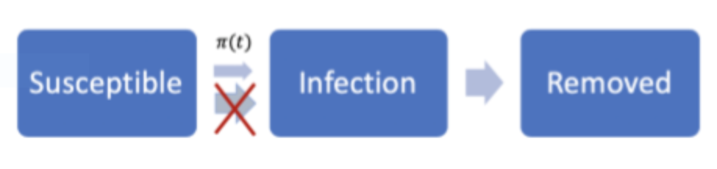
\includegraphics[width=6.38in]{figures/1}

  上述模型中疾病传播率的修正因子\(\pi(t)\)是根据地区所采取的隔离措施而特别给定的,本文北京市具体政策情况如下图所示。

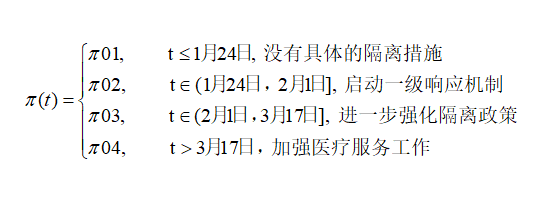
\includegraphics[width=7.42in]{figures/2}

  \(\pi(t)\)可选用两种函数形式,比较其进行修正后,与实际情况的偏差。
第一种为阶跃函数,可以反映不同时期政府采取的宏观隔离政策。当
\(\pi_{0}=(\pi_{01},\pi_{02},\pi_{03},\pi_{04})\)
选择不同的值时,疾病传播率也会不同。本次用的 \(\pi_{t}\)
分别为(1,1,1,1),(1,0.8,0.5,0.1),(1,0.9,0.7,0.5)。\(\pi(t)\)
第二种为连续函数,可以反映大众稳定增加的自我隔离意识和不断增加的隔离方法,相比于上面所讲的阶跃函数,这是从微观(个人)的角度来反映隔离效应。
\(\pi(t)\) 本文使用 \(\lambda_0=0.05\) 时的指数函数,具体函数形式如下。
\[ \pi(t)=exp(-\lambda_0t) 或者 \pi(t)=exp\lbrace-(\lambda_0t)^v\rbrace \]

  当\(\pi_{t}=(1,1,1,1)\)时,无政府干预,即体现自然状况下疫情的发展变化情况。

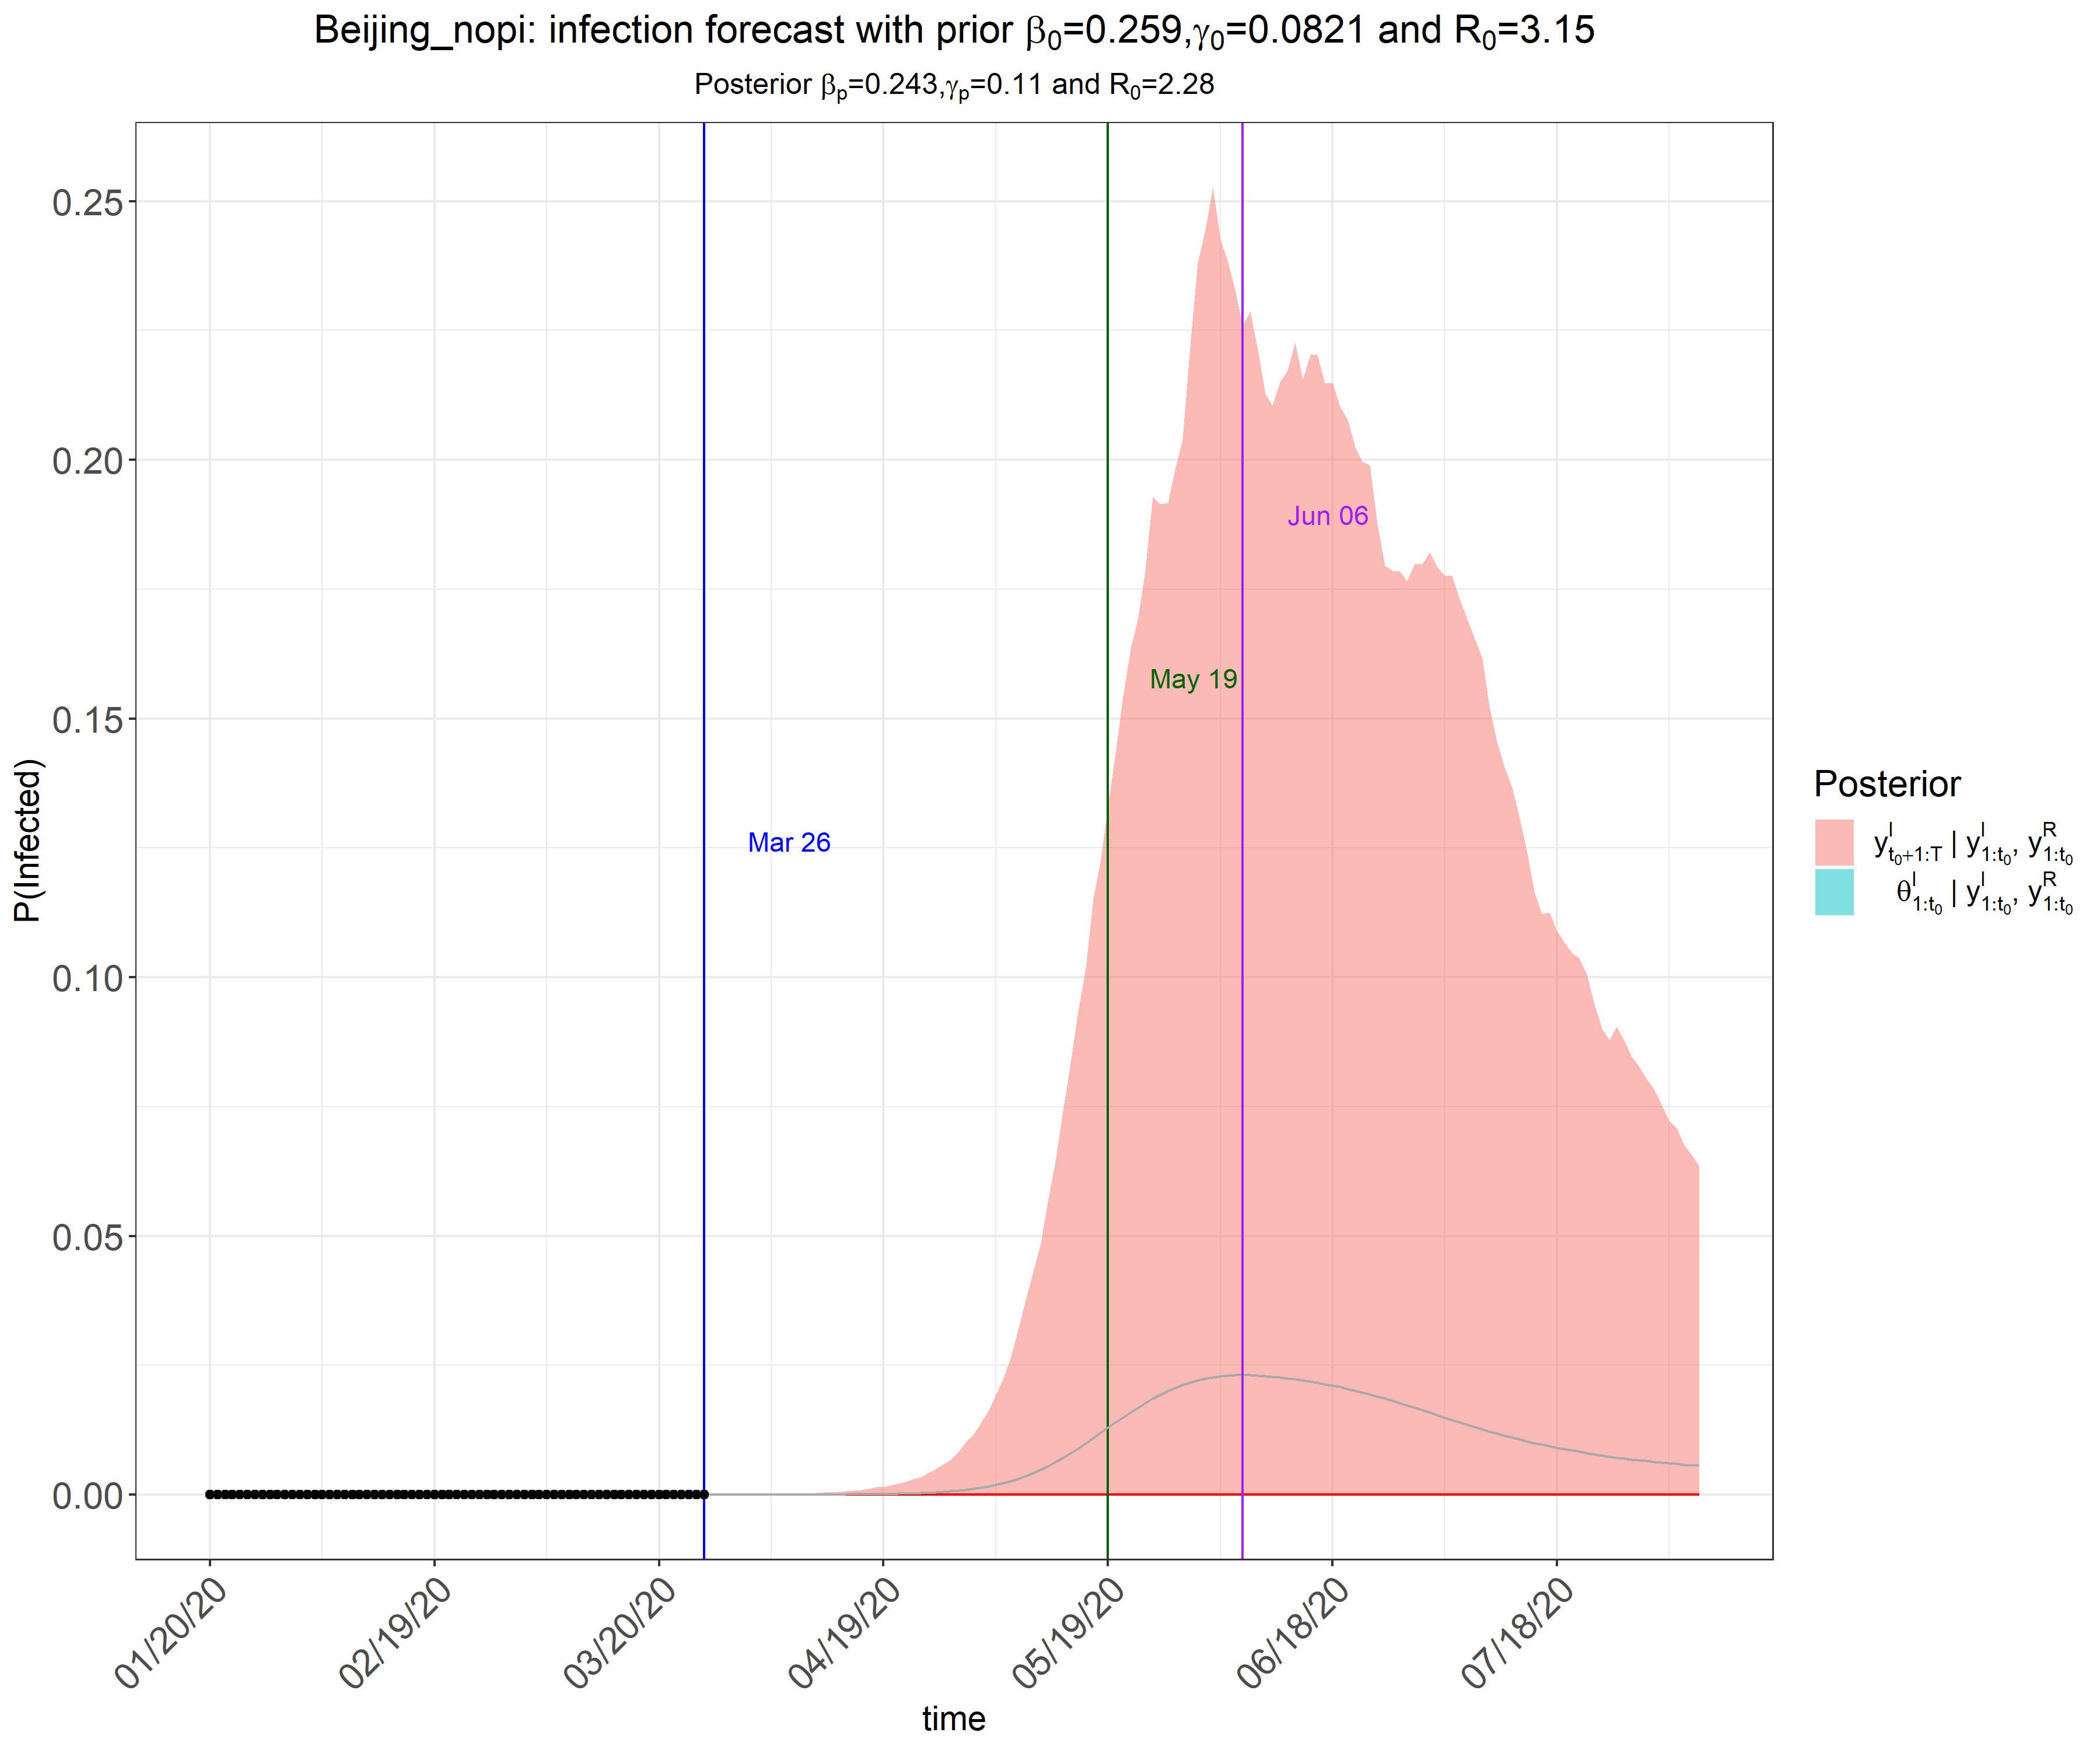
\includegraphics[width=50in]{figures/infection3}
  上图中蓝色竖线为原始数据拟合和预测数据的分界线,蓝色竖线以前为原始数据和其连续化拟合线。绿色竖线为第一拐点,粉紫色竖线为第二拐点。绿色曲线为数据均值,红色曲线为中值。由上图我们可以看出,若政府不对疫情进行干预,降低疾病传播率;北京市疫情仍有再次爆发的可能性。故在当前积极复工复产的同时,也要有效抑制疾病的传播。

  通过比较\(\pi_{t}\)的不同取值,找寻更符合北京市政策力度的赋权方式。

  当\(\pi_{t}=(1,0.8,0.5,0.1)\)时,疫情预测情况如下。

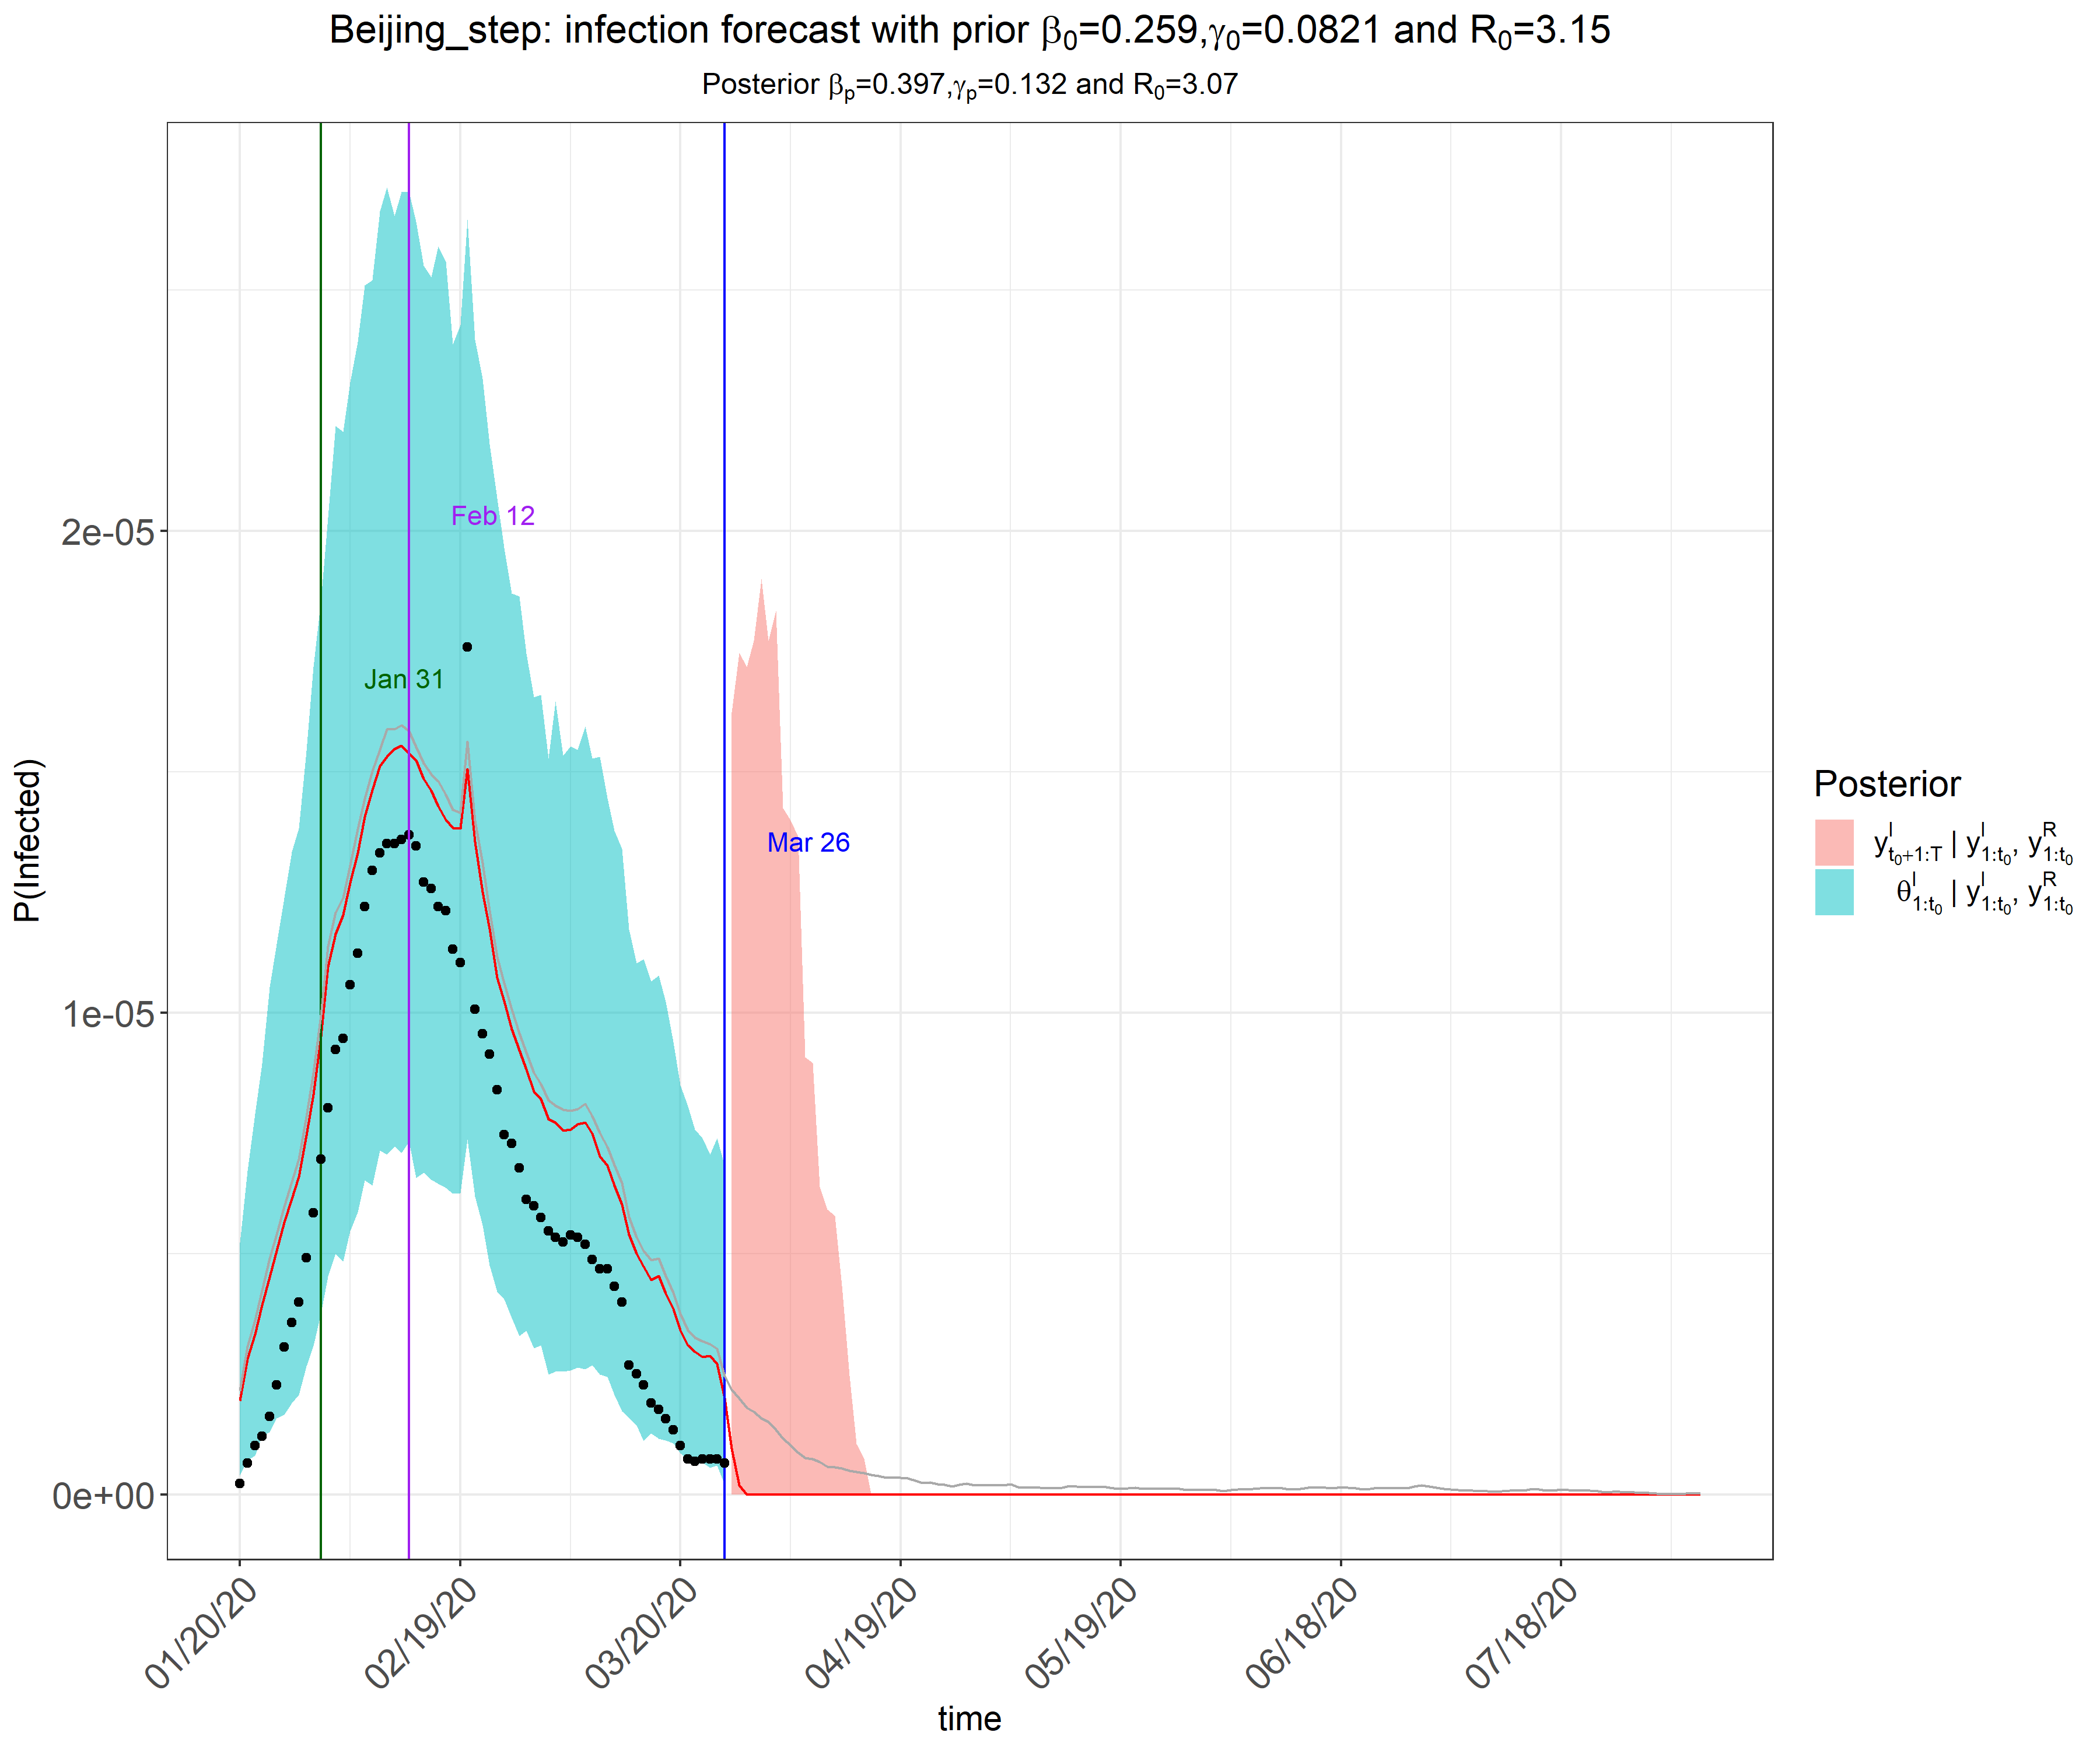
\includegraphics[width=50in]{figures/infection1}

  上图中,黑点为原始数据;对原始连续化处理进行进一步预测。在实际数据中,第一拐点为2月4日,第二拐点为2月12日。而在本次赋权分析中,第一拐点为1月31日,第二拐点与实际情况吻合。当感染人数曲线与y轴相切时;为第三拐点,疫情基本结束。在上图的预测部分,感染人数比例持续下降,直至为零;这与当前北京市除输入型病例的疫情情况较为吻合。该赋权方法,较为有效地体现了北京市不同政策力度情况。

  当\(\pi_{t}=(1,0.9,0.7,0.5)\)时,疫情预测情况如下。

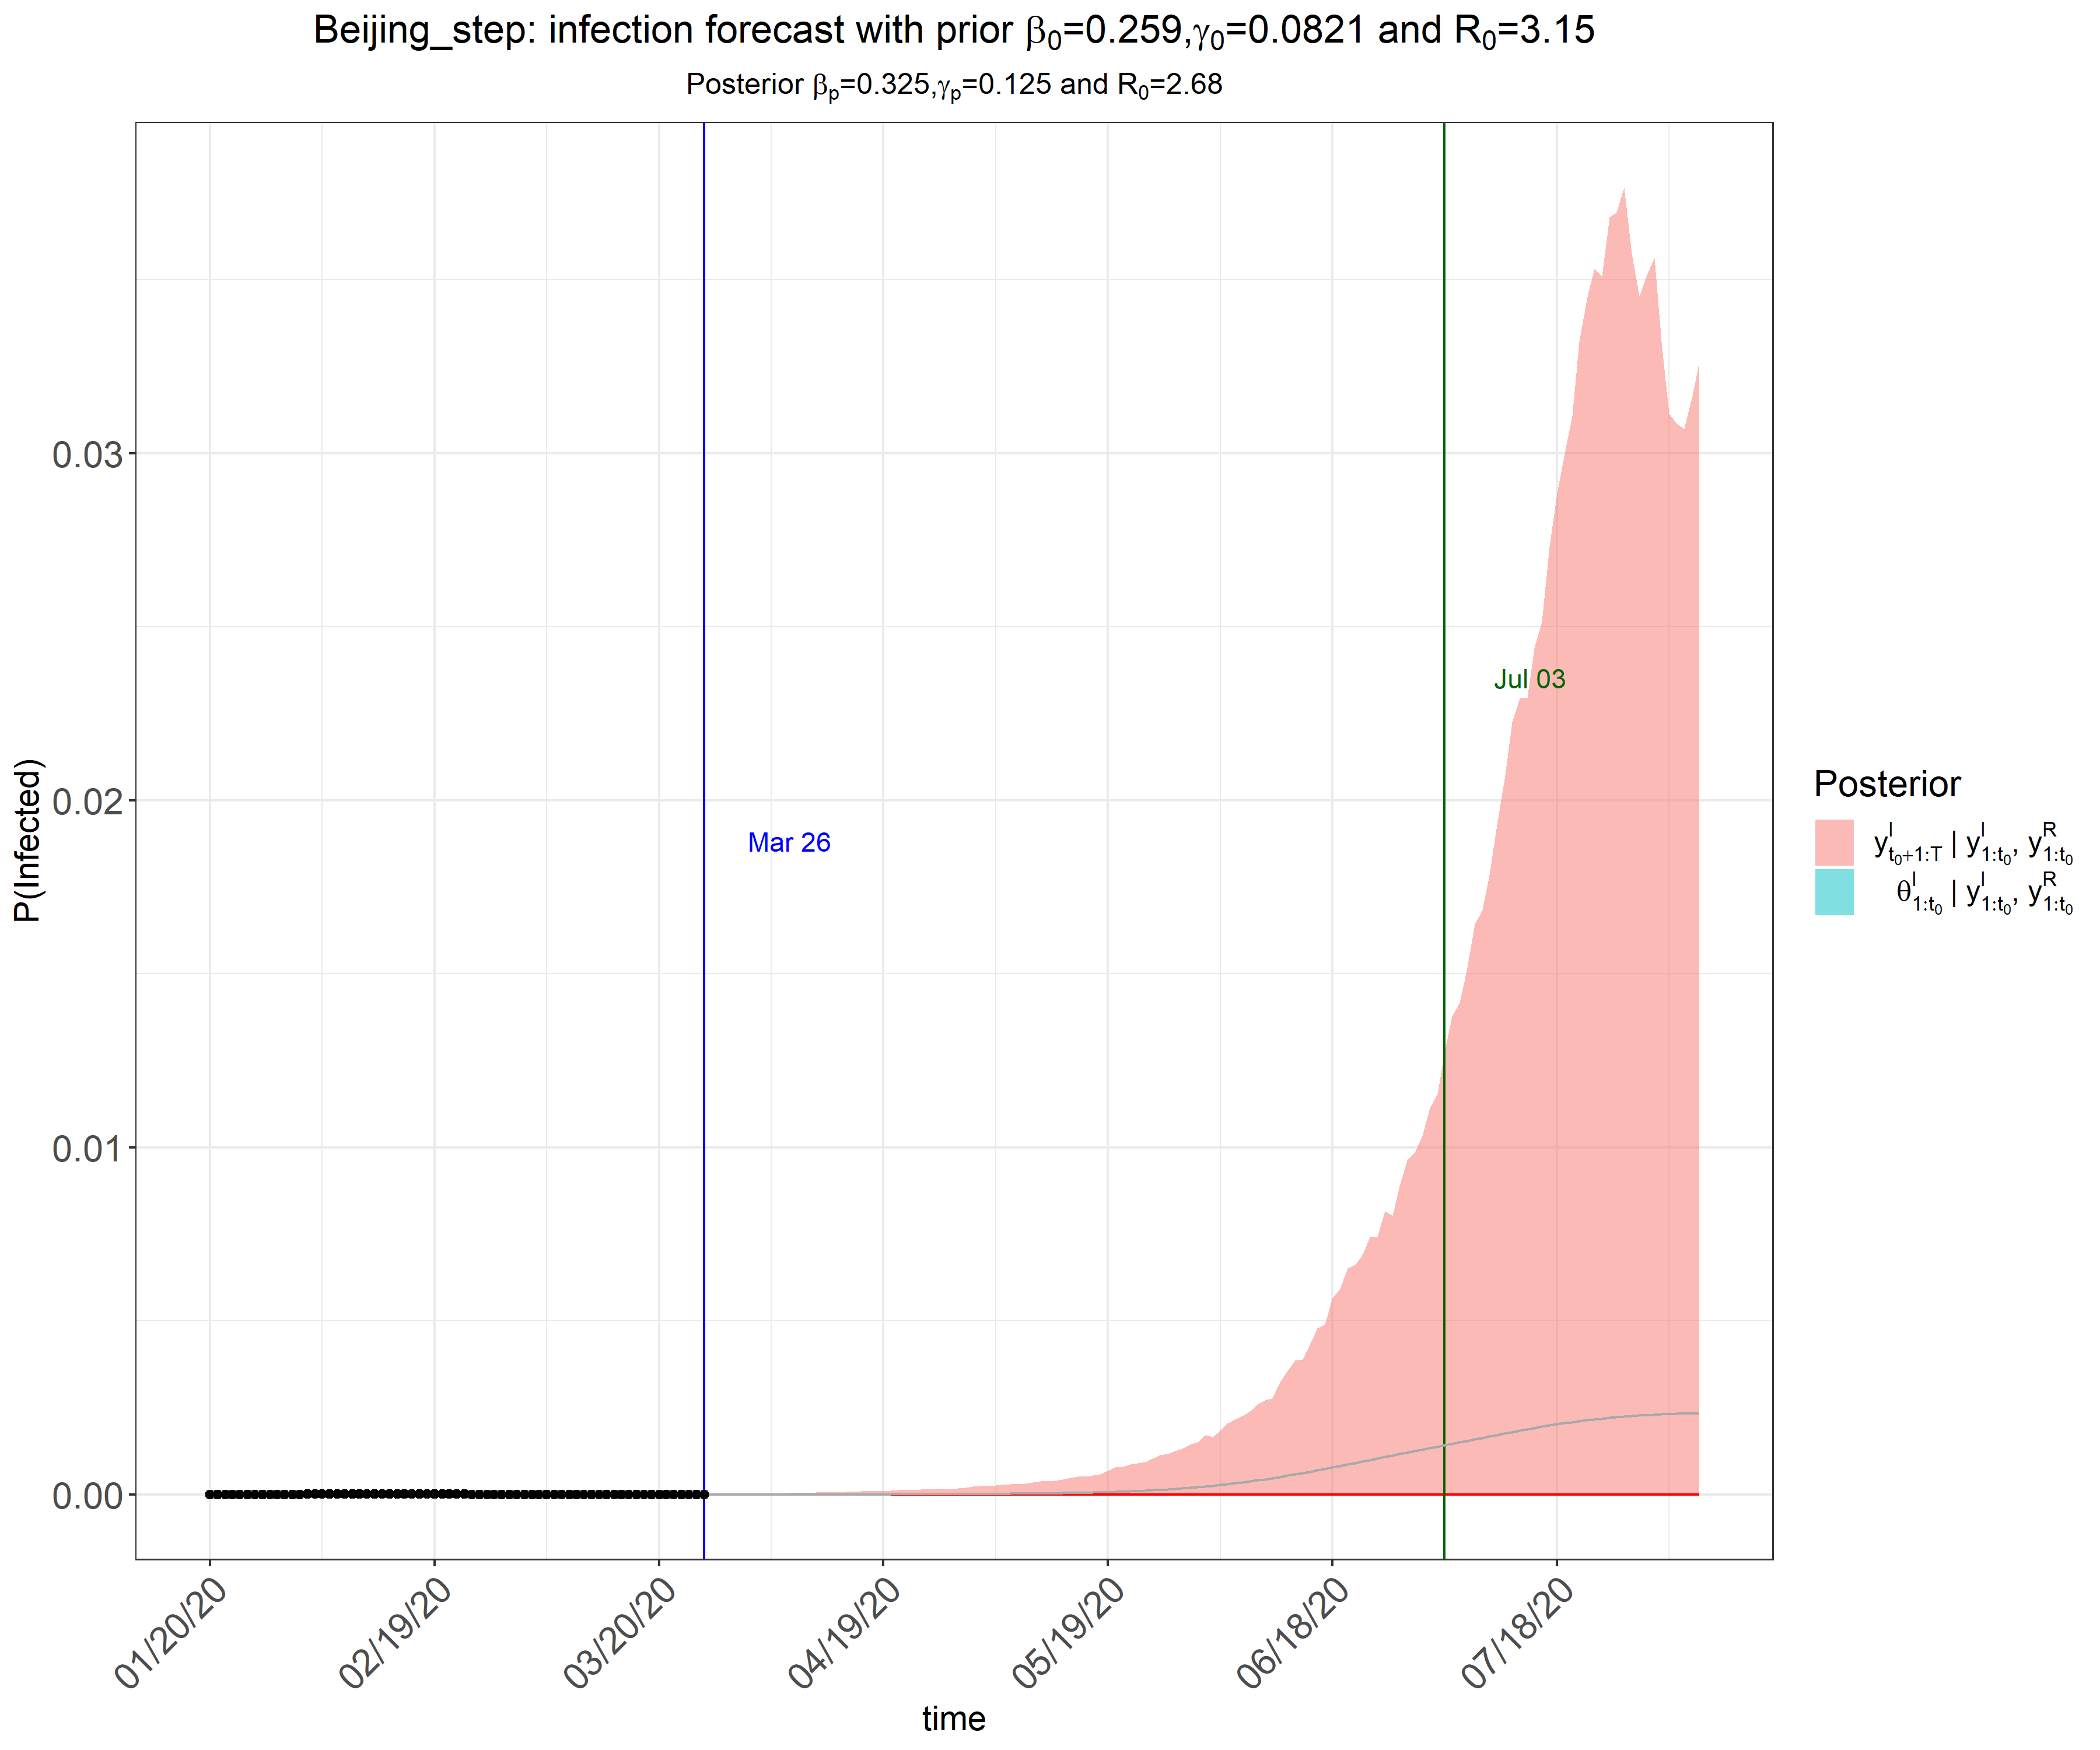
\includegraphics[width=50in]{figures/infection2}

  上图中,按照该赋权方法,疫情会在5月中后旬再次爆发;与当前实际情况不符。该赋权没有有效体现北京市政策对疫情的干预情况。

  当\(\pi(t)=exp(-0.05t)\)时,疫情预测情况如下。

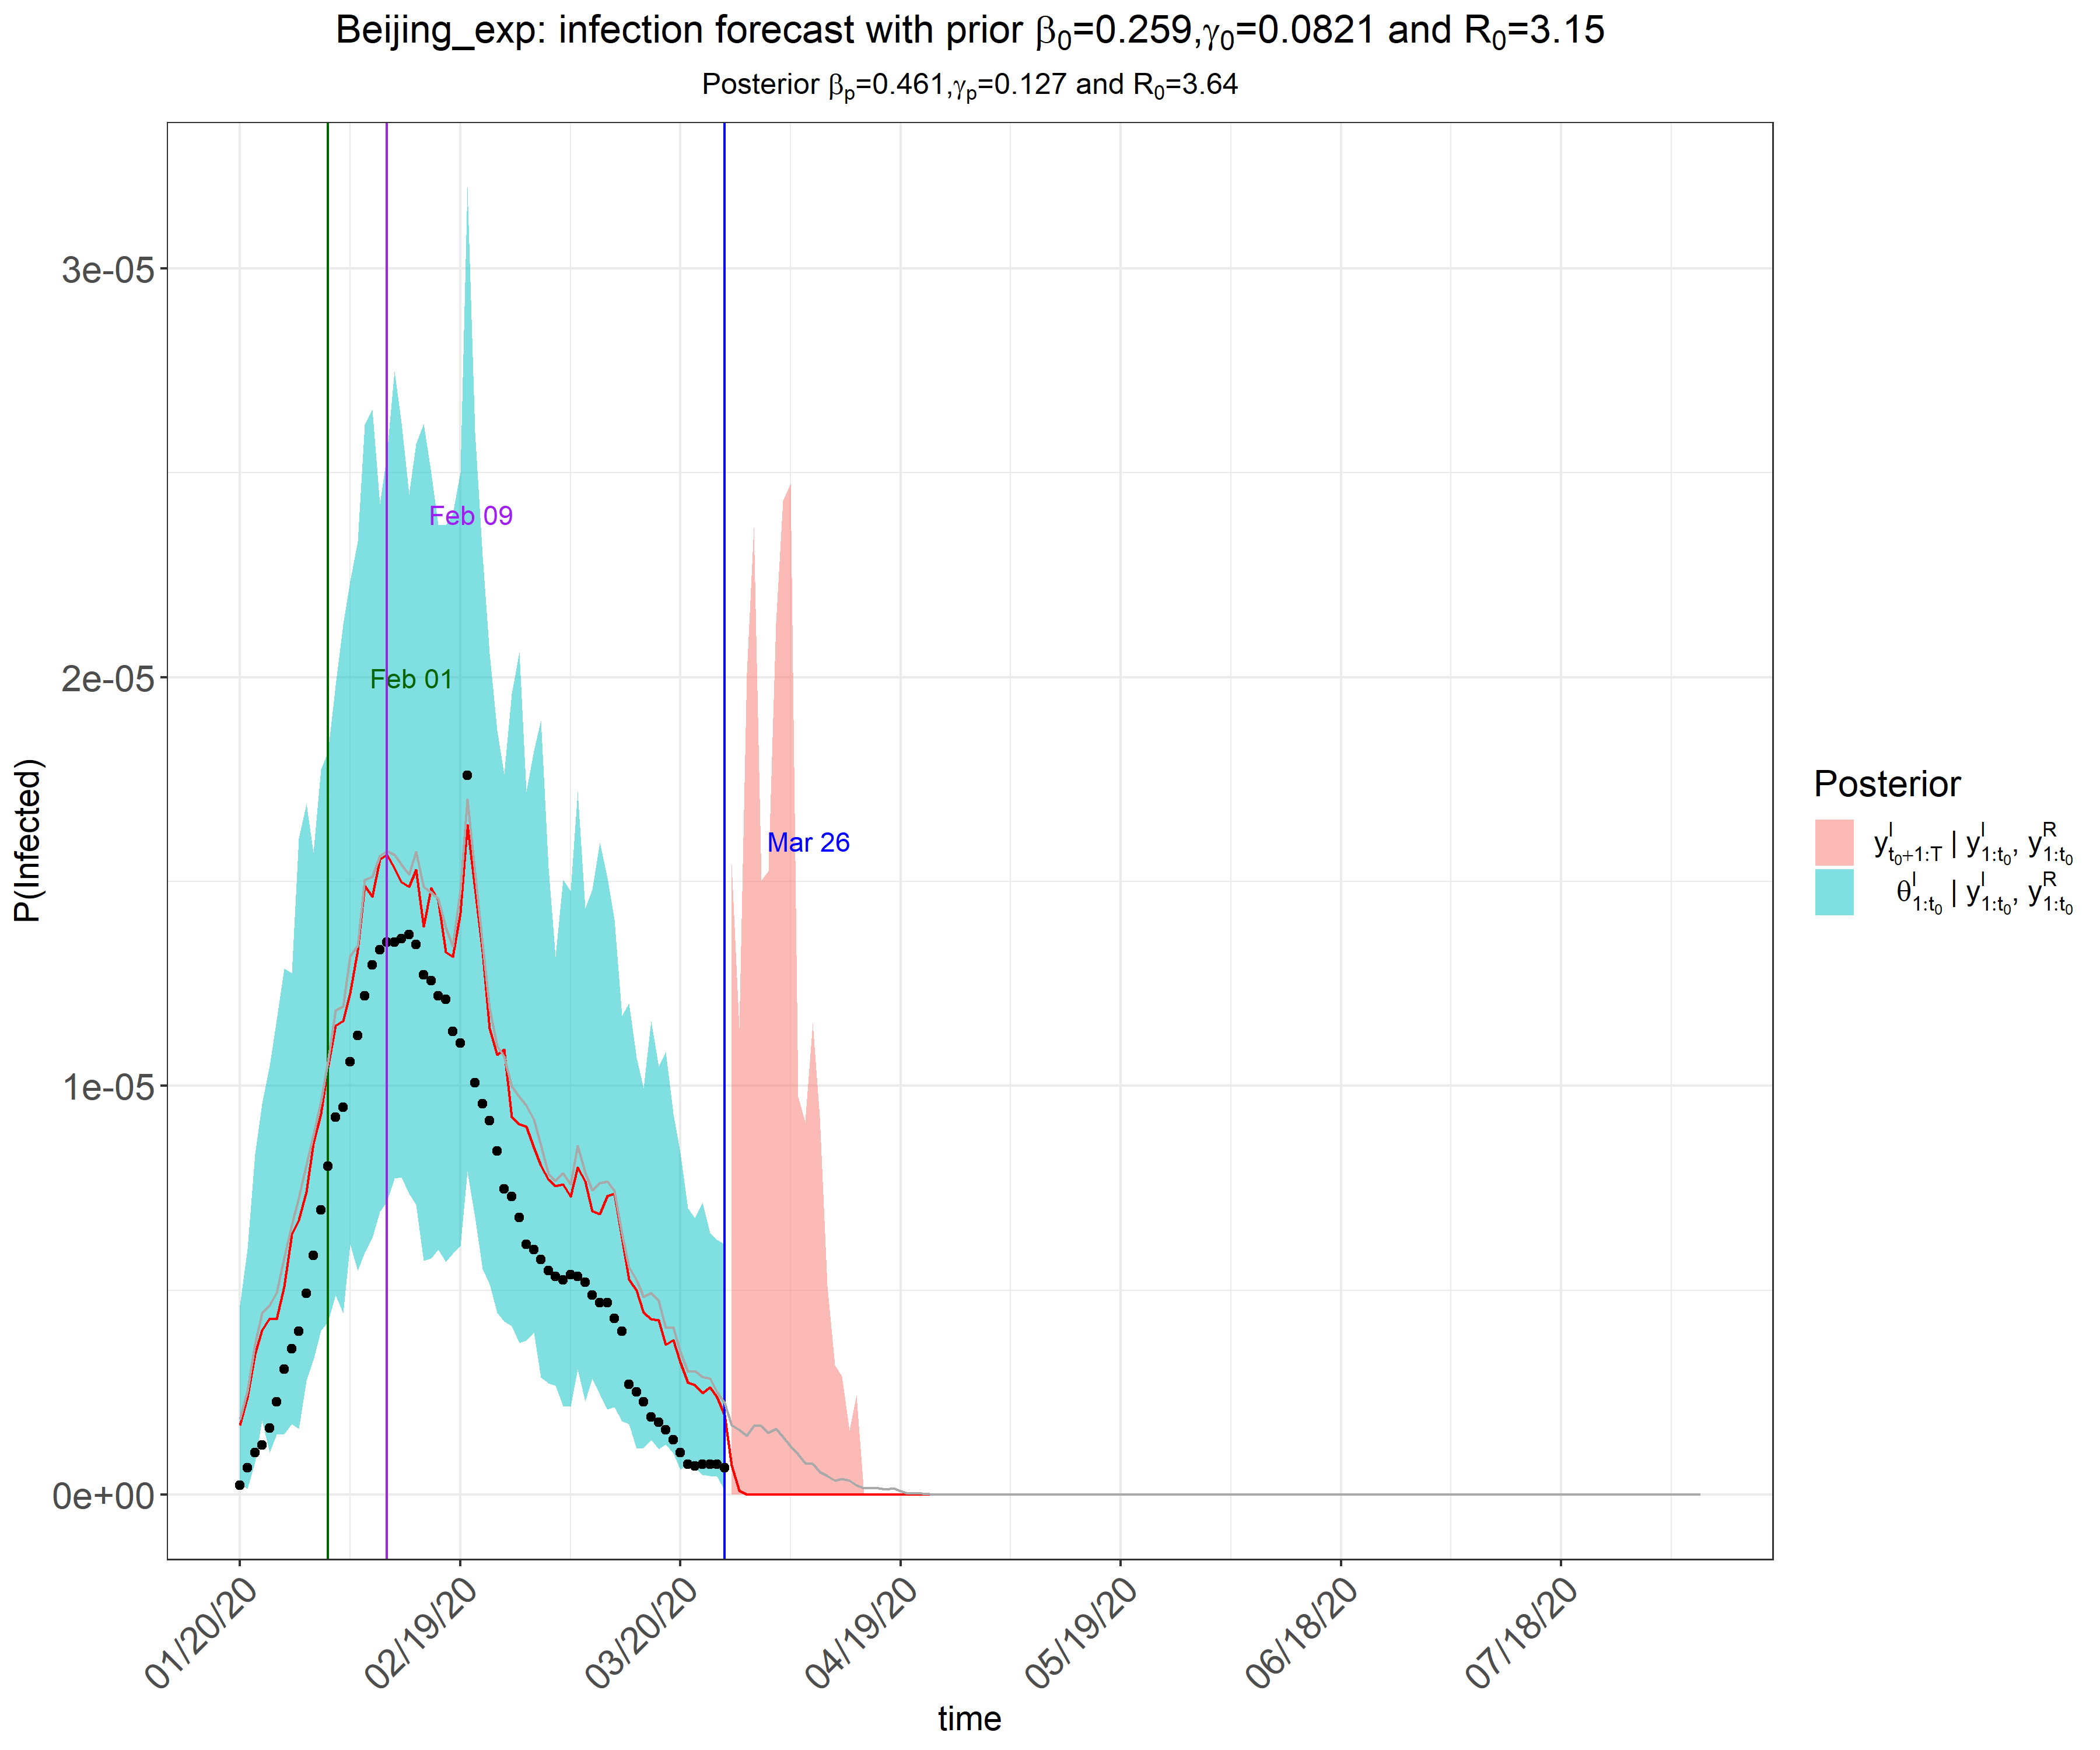
\includegraphics[width=50in]{figures/infection5}

  在本次赋权分析中,第一拐点为2月1日,第二拐点为2月9日;与实际拐点日期存在差异,但差异不大。第三拐点也在3月底出现,与实际情况较为符合。在上图的预测部分,感染人数比例保持总体下降趋势,但有一定向上增长的波动。该波动与实际情况存在较大差异,该赋权方法,体现了北京市不同政策力度情况,但对政策力度的界定不够准确。

  通过比较\(\pi(t)\)不同取值,对北京疫情情况的预测;得出\(\pi_{t}=(1,0.8,0.5,0.1)\)可以较好体现政策干预力度。1月24日启动一级响应机制,实施交通管制可以降低20\%的疾病传播率;2月1日进一步强化隔离政策,疾病传播率较原来相比降低了50\%左右。3月17日,在隔离政策的基础上,加强医疗服务;使得疾病传播率大幅度下降,仅为自然状态下疾病传播率的10\%左右。

\hypertarget{ux5212ux5206ux9694ux79bbux533aux7684ux62d3ux5c55ux7684sirux6a21ux578b}{%
\paragraph{4.4划分隔离区的拓展的SIR模型}\label{ux5212ux5206ux9694ux79bbux533aux7684ux62d3ux5c55ux7684sirux6a21ux578b}}

  上一个模型是在原有SIR模型的基础上引入 \(\pi(t)\)
修正因子,修正了易感染者接触感染者的概率,得到了新的SIR模型。本小节是在原有模型的基础上引入隔离区,如下图所示:

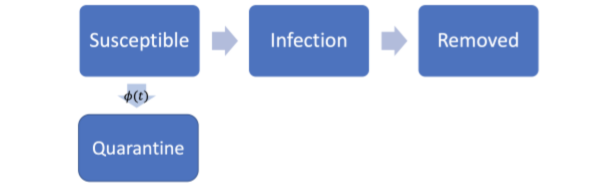
\includegraphics[width=8.24in]{figures/3}

该模型引入了Quarantine(隔离区),通俗的认为隔离区内的人是不会与感染者直接接触的人。
\(\phi(t)\)用于表示易感者愿意在t时刻在家自我隔离的概率,同上面所讲的一样,它也会随着时间而变换。因此,新的扩展SIR模型如下:

\[\frac{d{\theta_t}^I}{dt}=\beta{\theta_t}^S {\theta_t}^I -\gamma {\theta_t}^I, \frac{d{\theta_t}^S }{dt} =-\beta {\theta_t}^S {\theta_t}^I -\phi(t){\theta_t}^S\]

\[\frac{d{\theta_t}^Q}{dt}=\phi(t){\theta_t}^S,\frac{d{\theta_t}^R }{dt} = \gamma{\theta_t}^I\]

以上公式中 \({\theta_t}^S+{\theta_t}^Q+{\theta_t}^I+{\theta_t}^R=1\)

假定 \(\phi(t)\)
是狄拉克函数,并根据实际情况指定如下函数来反映宏观干预政策的影响:

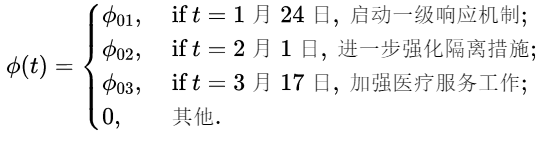
\includegraphics[width=7.78in]{figures/4}

令
\(\phi_{0} =(\phi_{01},\phi_{02},\phi_{03})\),本文考虑了两种情况:有多个温和跳跃点(
\(\phi_{0}=(0.1,0.4,0.4)\))和仅有一个大的跳跃点(\(\phi_{0}=(0,0.9,0)\)
)的情况。

当\(\phi_{0}=(0.1,0.4,0.4)\)时,疫情预测情况如下:

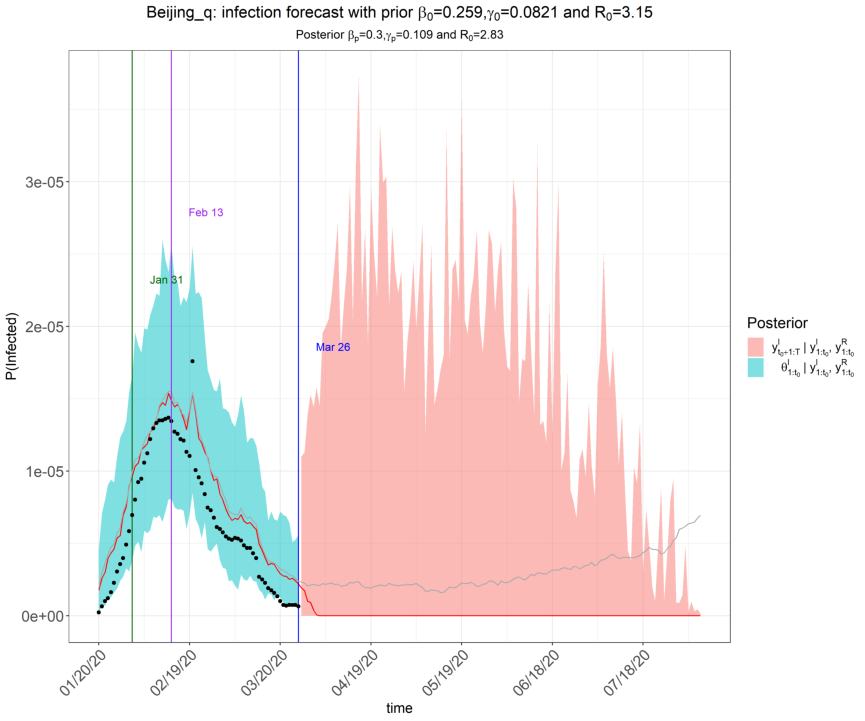
\includegraphics[width=50in]{figures/q11}

从上图可以看出,在本次赋权分析中,第一拐点为1月31日,第二拐点为2月13日,这与实际情况吻合。三月底为第三拐点,疫情基本结束。在上图的预测部分,观察绿色曲线,感染人数比例在6月会小规模二次爆发,这与当前北京市当前疫情情况较为吻合。

当\(\phi_{0}=(0,0.9,0)\)时,疫情预测情况如下:

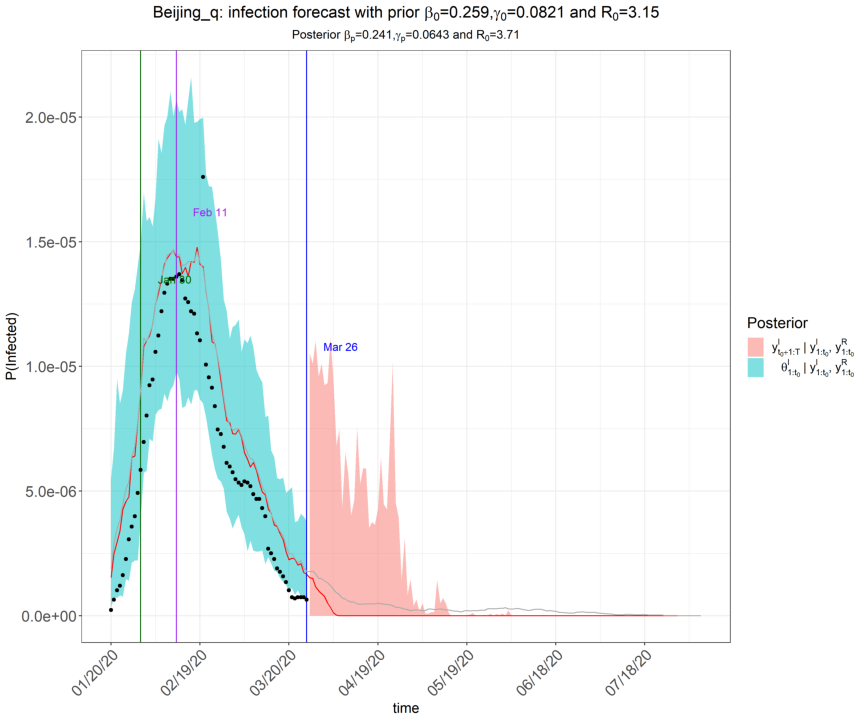
\includegraphics[width=50in]{figures/q21}

从上图可以看出,在本次赋权分析中,第一拐点为1月30日,第二拐点为2月13日,这与上面模型基本没有区别。4月5日左右为第三拐点,表示疫情基本结束。感染人数比例保持总体下降趋势,但有一定向上增长的波动。

\hypertarget{ux4e94ux7ed3ux8bbaux4e0eux5c55ux671b}{%
\subsubsection{五、结论与展望}\label{ux4e94ux7ed3ux8bbaux4e0eux5c55ux671b}}

\hypertarget{ux7ed3ux8bba}{%
\paragraph{5.1结论}\label{ux7ed3ux8bba}}

  通过两种改进模型的分析,结合北京实际疫情描述统计,拓展的SIR模型对北京疫情发展趋势的预测分析与实际较为符合。对于修正疾病传播率的SIR模型,本文中采取的\(\pi_{t}=(1,0.8,0.5,0.1)\)赋权方式相比于另外几个赋权与北京市的疫情情况较为吻合,有效体现了北京市不同政策力度情况。对于划分隔离区的SIR模型,本文采取的赋权方式基本也符合北京市的情况,与各个拐点基本吻合。从中我们可以知道,政府采取相关干预措施和政策对于新型冠状病毒的流行控制是非常有效和有必要的,能够较短时间内控制疫情,保障人民生命财产安全。另外相关的改进传染病模型对于疫情的预测也是有效的;选择合适的赋权方式对疫情预测对于疫情的防控和政策的制定意义非凡。

\hypertarget{ux5c55ux671b}{%
\paragraph{5.2展望}\label{ux5c55ux671b}}

  本文中主要运用了基础SIR模型改进的两种:修正疾病传播率的SIR模型和划分隔离区的拓展SIR模型。对于基础SIR模型的改进还有很多种,皆是为了能更好的结合实际人们面对传染病做出行动而做出更好的拟合和预测。接下来可以考虑的是在划分隔离区的拓展SIR模型的基础上加入住院舱室,针对已感染人群隔离住院室,即既有隔离室又有住院室的模型;或者加入疑似感染人群的SIR模型。\\
  另外,对于政府政策干预的改进模型,政策的实施对于模型中赋权是还需考虑的一个问题,本文中对两个改进模型各选用两至四个赋权方式来比较哪种方式更符合北京市实际情况,而根据组合可以有很多赋权方式,通过不断的赋权,找到内在依据和规律以更好的预测是接下来的方向。

\hypertarget{ux516dux53c2ux8003ux6587ux732e}{%
\subsubsection{六、参考文献}\label{ux516dux53c2ux8003ux6587ux732e}}

{[}1{]}An epidemiological forecast model and software assessing
interventions on COVID-19 epidemic in China.

{[}2{]}Canrong Tian,Qunying Zhang,Lai Zhang. Global stability in a
networked SIR epidemic model{[}J{]}. Applied Mathematics
Letters,2020,107.

{[}3{]}COVID-19/SARS-CoV-2 News from Preprints; An Age and Space
Structured SIR Model Describing the Covid-19 Pandemic{[}J{]}. Medical
Letter on the CDC \& FDA,2020.

{[}4{]}Pegah Taghiei Karaji,Nemat Nyamoradi. Analysis of a fractional
SIR model with General incidence function{[}J{]}. Applied Mathematics
Letters,2020,108.

{[}5{]}李贻芬.传染病传播模型的探究及优化运用{[}J{]}.通化师范学院学报,2019,40(08):26-31.

{[}6{]}种大双,孙绍荣.基于传染病模型的重大突发事件舆情传播与控制{[}J{]}.情报理论与实践,2018,41(05):104-109.

{[}7{]}朱仁杰,唐仕浩,刘彤彤,等.基于改进SIR模型的新型冠状病毒肺炎疫情预测及防控对疫情发展的影响.

{[}8{]}喻孜,张贵清等. 基于时变参数-SIR 模型的2019-nCoV疫情评估和预测

{[}9{]}许云霞,雷学红.具有Logistic增长的SIRS传染病模型的稳定性及最优控制分析{[}J{]}.湖北民族大学学报(自然科学版),2020,38(02):200-205.

\end{document}
